\chapter{Architektur}
\label{architektur}

Das Gesamtsystem setzt sich aus insgesamt vier Komponenten zusammen: die Datenbank, der Webserver, die Fehlerquelle und das Zielsystem von \gls{OpenStreetMap}. 
Die einzelnen Komponenten sind über \gls{REST}-Schnittstellen miteinander verbunden. 
Dabei sind das Zielsystem (\gls{OpenStreetMap}) und die Fehlerquelle (\emph{KeepRight}, siehe Kapitel \ref{datenquellen}) Fremdsysteme, bei welchen die Schnittstellen gegeben waren. 
Unsere eigenen Server haben wir entsprechend angepasst und auch via \gls{REST} zugänglich gemacht.

\begin{figure}[H]
	\centering
	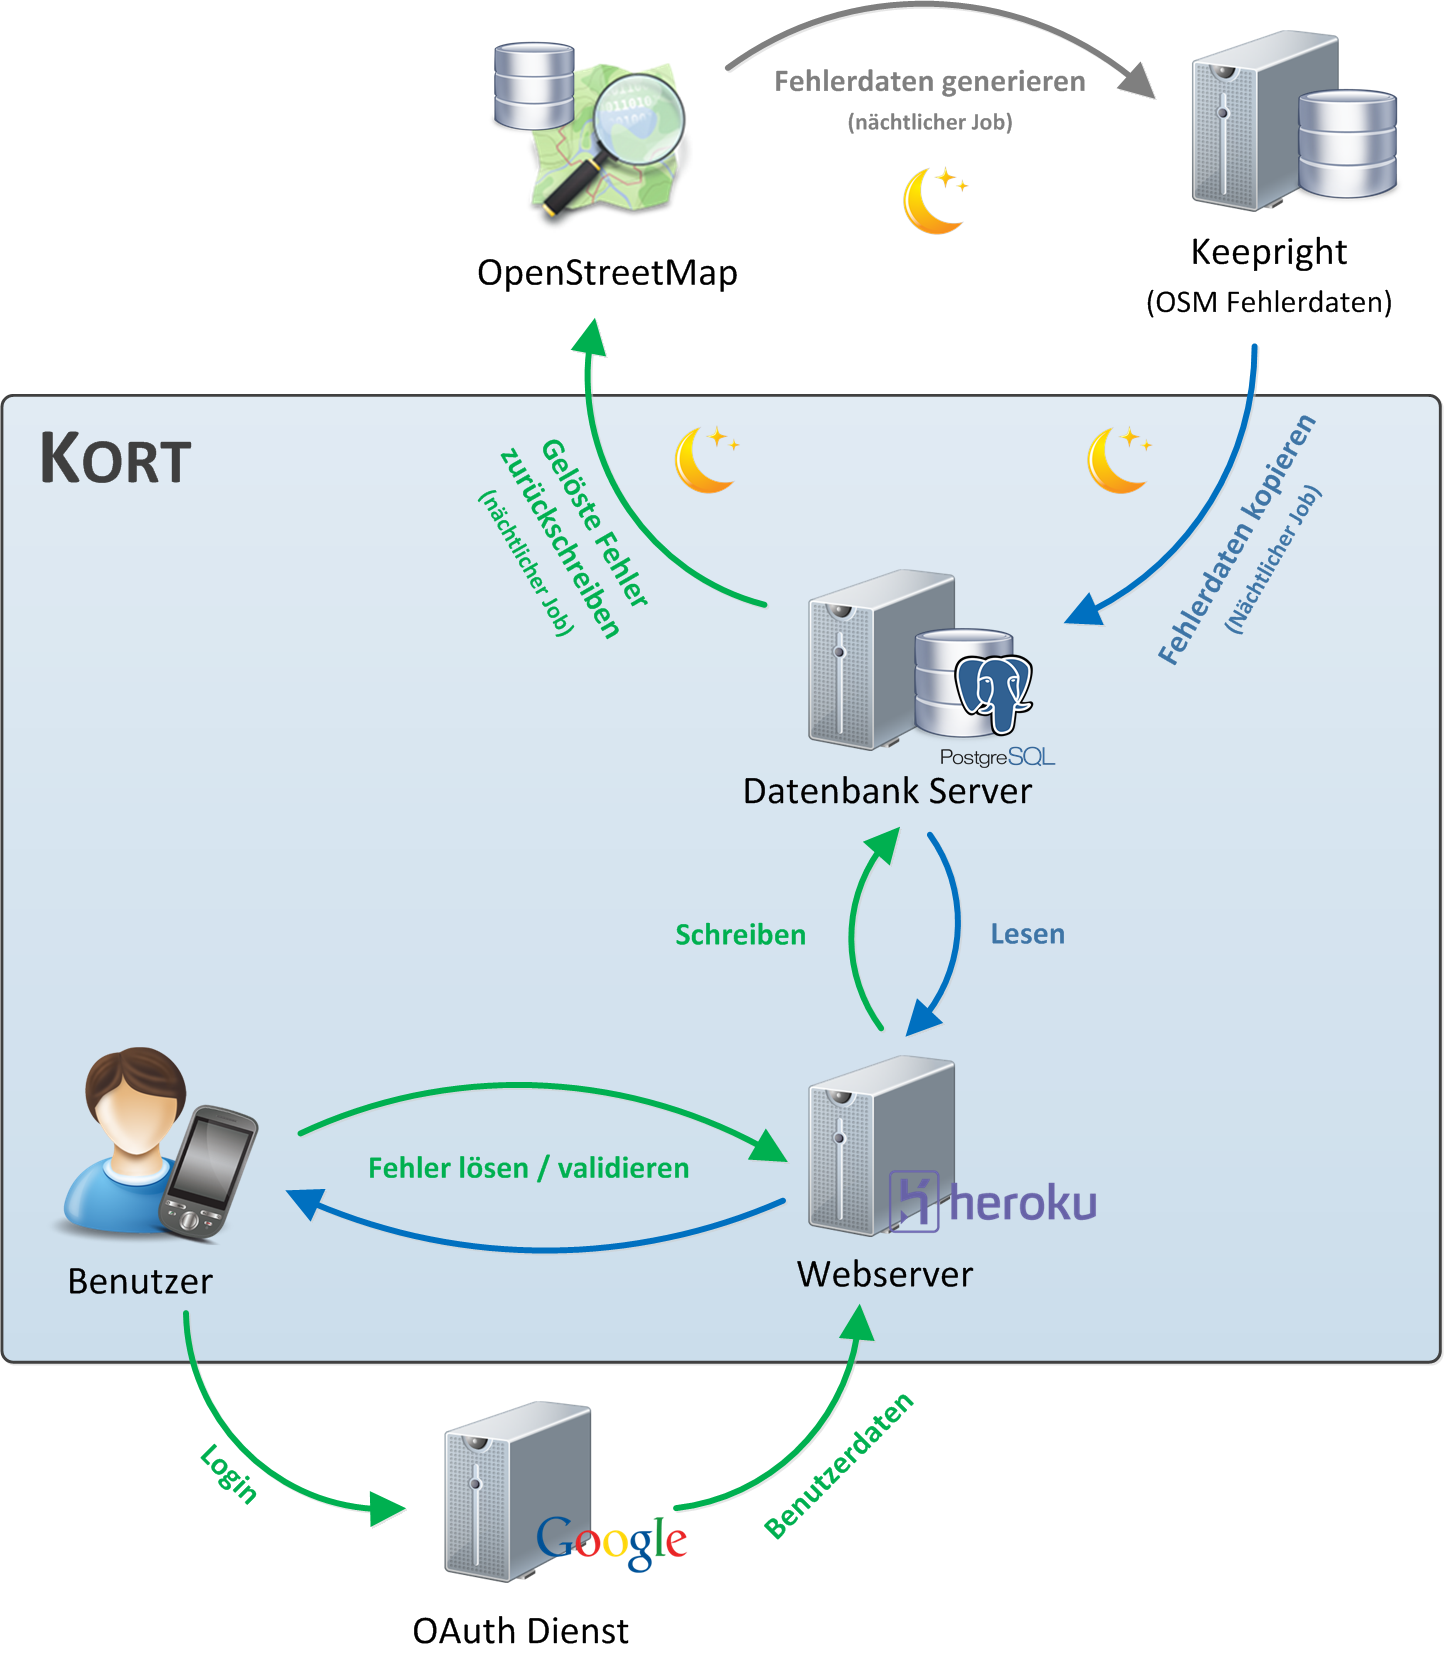
\includegraphics[scale=0.32]{images/implementation/backend/kort-big_picture}
	\caption{Übersicht des Gesamtsystems}
	\label{image-kort-big-picture}
\end{figure}

Das Backend besteht aus zwei logisch und derzeit auch physisch getrennten Servern. 
Der Webserver liefert die \gls{WebApp} aus und ist auch der einzige Kommunikationspartner für das Frontend. Dies ist zum einen eine architektonische, zum anderen eine technische Entscheidung.

\begin{itemize}
\item Das Frontend muss sich nicht darum kümmern woher es welchen Dienst bezieht
\item Die Same-Origin-Policy\cite{sop} einiger Server lässt keine direkte Kommunikation zwischen \emph{fremdem} JavaScript und dem Server zu
\end{itemize}

Der Webserver ist somit der Dreh- und Angelpunkt der Applikation, jegliche Informationen von und zum Frontend durchläuft diese zentrale Komponente.

\begin{figure}[H]
	\centering
	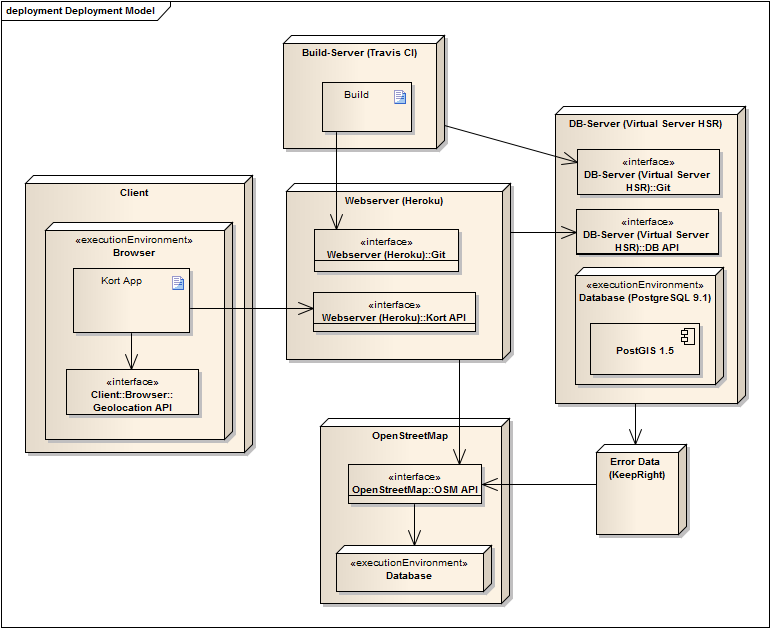
\includegraphics[width=\textwidth]{images/uml/deployment_diagram}
	\caption{Deployment-Diagramm}
	\label{deplyoyment-diagram}
\end{figure}

\section{Bootstrapping}
Das \gls{Bootstrapping} ist ein sehr wichtiges Grundprinzip dieser Arbeit.
Es besagt, dass sich das System selbst aufbauen kann.
Konkret haben wir darauf geachtet, dass für alle Aktionen Skripte oder Build-Schritte vorhanden sind, um diese später nachzuvollziehen.
Dies Ziel ist es, ein System zu entwickelt, dass sich möglichst einfach wieder aufbauen lässt.

Auf der Seite des Datenbankserver geschieht dies so, dass die Datenbank jede Nacht neu aufgebaut wird.
Zum einen werden dabei die neuesten Fehlerdaten von \emph{KeepRight} geladen, zum anderen alle Änderungen an der Datenbank nachvollzogen.
Dies hat den grossen Vorteil, dass stets ein konsistenter Zustand anzutreffen ist.

Eine Ausnahme bilden dabei die laufenden Daten der Applikation (d.h. Userdaten, Lösungsvorschläge etc.), welche nicht jede Nacht zurückgesetzt werden.
Dies hat aber eher praktische als technische Gründe.

Auf der Seite des Webservers ist dies das \gls{Bootstrapping} noch stärker anzutreffen, da bei jedem Build tatsächlich das System komplett neuaufgebaut wird.
Somit müssen alle Informationen in Skripten hinterlegt sein, da sie sonst schlicht nicht zur Anwendung kommen.

\section{Umsysteme}
Zu unserem System gehören auch die Fehlerdatenquelle \emph{KeepRight} sowie \gls{OpenStreetMap} dazu.
Unsere Applikation interagiert direkt mit diesen beiden Systemen, ohne eine Kontrollfunktion zu übernehmen.
Es handelt sich somit um sogenannte Fremdsysteme.

Bei der Gestaltung der Systemlandschaft war es uns wichtig, diese so flexibel und offen wie möglich zu gestalten.
Weitere Systeme sollen sich einfach Einbinden lassen.
Um dieses Ziel zu erreichen haben wir darauf geachten keine festen Verbindungen zwischen den Systemen zu schaffen.
Solche lassen sich später nur schwer wieder entfernen oder ändern.

Ein wichtiger Eckpfeiler ist auch, die gesamte Kommunikation über \gls{REST}-Schnittstellen zu realisieren.
Dadurch lassen sich Dienste sowohl orts- wie auch technologie-unabhängig voneinander betreiben.

\subsection{KeepRight}
Die Verbindung zu \emph{KeepRight} ist sehr lose, da das angebotene \gls{API} lediglich ein täglich generierter Dump von Fehlerdaten ist.
Diese Daten werden jede Nacht heruntergeladen und in unsere Datenbank integriert.

Weitere Fehlerquellen lassen sich einfach einbinden (siehe Abschnitt \ref{additional-error-source}), da innerhalb der Applikation nur über eine View auf die Daten zugegriffen wird.

\subsection{OpenStreetMap}
Das System benötigt drei Schnittstellen zu \gls{OpenStreetMap}, wovon in dieser Arbeit zwei realisiert sind.

\gls{OpenStreetMap} liefert die genauen Informationen über ein geografisches Objekt, um dieses auf einer Karte zeichnen zu können.
Dies verwenden wir um Details zu einem Fehler anzuzeigen.
Wenn beispielsweise der Name einer Strasse erfasst werden soll, kann sich der Benutzer vorher über die Detail-Karte darüber vergewissern, welche Strasse genau gemeint ist.

Der zweite Dienst, den wir beanspruchen ist die Authentifizierung über \gls{OAuth}.
So kann das \gls{OpenStreetMap}-Benutzerkonto direkt verwendet werden um \kort zu spielen.

Um den Kreis zu schliessen, sollen Korrekturen an \gls{OpenStreetMap} zurückgeschickt werden.
Dieses Themengebiet ist sehr heikel, da die \gls{OpenStreetMap}-Community gegenüber technischen Benutzern sehr kritisch gegenübersteht.
Es gilt die Grundregel, dass alle Änderungen über persönliche Benutzerkonten gemacht werden müssen.

Dies hat vor allem damit zu tun, dass Änderungen leicht nachvollziehbar sind.
Solche Einschränkungen können jedoch auch ein Hindernis sein.
In begründeten Fällen wird deshalb auch eine Ausnahme zugelassen.
Beispielsweise hat die \emph{WheelMap}-Applikation\footnote{\url{http://wheelmap.org/}} offiziell die Erlaubnis mit einem technischen Benutzer Änderungen zu erfassen.

Dies war unter anderem auch der Grund weshalb wir unser Projekt am OSM-Stammtisch in Zürich vorgestellt haben\footnote{\url{http://wiki.openstreetmap.org/wiki/DE:Switzerland:Z\%C3\%BCrich/OSM-Treffen\#36._OSM-Stammtisch}}.
Das Feedback war durchaus positiv, jedoch gab es starke Vorbehalte gegenüber unserem Vorhaben, die korrigierten und validierten Lösungen automatisiert an \gls{OpenStreetMap} zu senden.

Das Thema ist also sowohl technisch als auch organisatorisch als komplex einzustufen.
Dies war uns von Anfang an klar, weshalb wir diesen Punkt auch in unserem Risikomanagement (siehe Abschnitt \ref{risikomanagement}) behandelt haben.
Schlussendlich hat uns die Zeit gefehlt dieses Feature zu implementieren, weshalb \kort derzeit ein geschlossenes System ist, welches Lösungvorschläge für Fehlerdaten sammelt.

\section{Authentifizierung}
Bei jeder Applikation, welche Daten für verschiedene Nutzer speichert, stellt sich die Frage, wie sich die User anmelden sollen.
Die wichtigsten Kriterien dabei sind:

\begin{itemize}
\item Sicherheit
\item Einfachheit
\item Zielpublikum
\item Benötigte Zusatzdienste
\end{itemize}

Auf diese Kriterien hin, war für uns sofort klar, dass wir keine eigene Benutzerverwaltung machen wollten.
Ein App, die primär eine Ablenkung für einige Minuten sein soll, kann es sich nicht leisten den Benutzer durch die Eingabe von Anmeldedaten abzuschrecken.

Daneben hat ein Benutzer bereits sehr viele Benutzerkonten bei verschiedensten Diensten.
Daher ist es auch naheliegend diese Daten wiederzuverwenden.
Der Benutzer erspart sich dadurch einen weiteren Login, an den er sich erinnern muss und wir als Entwickler müssen uns nicht um die Anmeldung kümmern.

\Gls{OAuth} ist mittlerweile ein gängiger Standard, um Applikationen Zugriff auf fremde Resourcen zu geben, ohne direkt den Benutzernamen und das Passwort preiszugeben.
Auch \gls{OpenStreetMap} unterstützt \gls{OAuth} und so fiel die Entscheidung leicht, dieses Protokoll zu verwenden.

In unserem Fall ist die Resource jedoch \emph{nur} die Benutzerinformationen.
Das Protokoll basiert darauf, dass sowohl die Applikation, sowie der Benutzer dem jeweiligen \gls{OAuth}-Anbieter vertraut.

Vom authentisierten Benutzer werden dann die Benutzerinformationen (Name, ID, E-Mail) in unsere Datenbank übernommen.
Jeder Benutzer erhält daraufhin ein sogenanntes \emph{secret}, welches ihm fortan erlaubt ohne erneuten Login die App zu nutzen.
Eine genaue Erklärung des Login-Ablaufs wird in Abschnitt \ref{oauth} beschrieben.

\section{REST}
\GLS{REST} ist die Idealvorstellung von plattformunabhängigen Schnittstellen.
So lassen sich alle möglichen Entitäten als \emph{Resourcen} darstellen, welche über eine der vier Grundfunktionalitäten (\inlinecode{CRUD} - \inlinecode{Create}, \inlinecode{Read}, \inlinecode{Update}, \inlinecode{Delete}) manipuliert werden können.

Jede grössere Applikation kann von dieser Flexibilität profitieren.
Sie ermöglicht es, dass Funktionalitäten mit beliebigen Technologien und Programmiersprachen entwickelt werden können.
Dies ist besonders gut umsetzbar, wenn die Applikation bereits in Betrieb ist.
So können einzelne Komponenten neu entwickelt werden und in das bestehende System integriert werden ohne eine nennenswerte Downtime.

Beim Marshalling der Daten mag es effizientere Möglichkeiten geben als \inlinecode{JSON} und \inlinecode{XML}.
Wenn die Datenmengen gering sind, fällt dies jedoch nicht stark ins Gewicht.
Sobald Binärdaten übertragen werden müssen, könnte es sinnvoll sein, einige Komponenten über andere Schnittstellen anzusprechen.

In unserem System spielt das kein Rolle, da unsere Requests durchschnittlich 10KB gross sind.